% ===============================
%        Optics Measurements
% ===============================

\subsection{Turn by Turn}

\lipsum[1-2]





% ================================================= 
%                   Chromaticity
\subsection{Chromaticity}

% --- Procedure ---
\subsubsection{Procedure}

Chromaticity measurements are typically performed by varying the RF frequency to induce a change of momentum offset $\delta$, while measuring the tune.
The momentum offset $\delta$ being related to the RF frequency and the momentum compaction factor $\alpha_c$:

\begin{equation}
    \delta = - \frac{1}{\alpha_c} \cdot \frac{\Delta f_{RF}}{f_{RF,nominal}}
    \label{eq:dpp_rf}
\end{equation}

Frequency steps of 20Hz every 30 secondes are typically taken to compromise between number of data points, precision of the tune estimate, and duration of the measurement.
Once beam losses, registered by the Beam Loss Monitors (BLM), are deemed too high, the frequency is reverted back to its nominal value in larger steps. The same procedure is then re-applied in the negative. Figure \ref{fig:measurements:rf_scan} shows a typical RF scan performed to measure chromaticity in the LHC.

\begin{figure}[H]
    \centering
    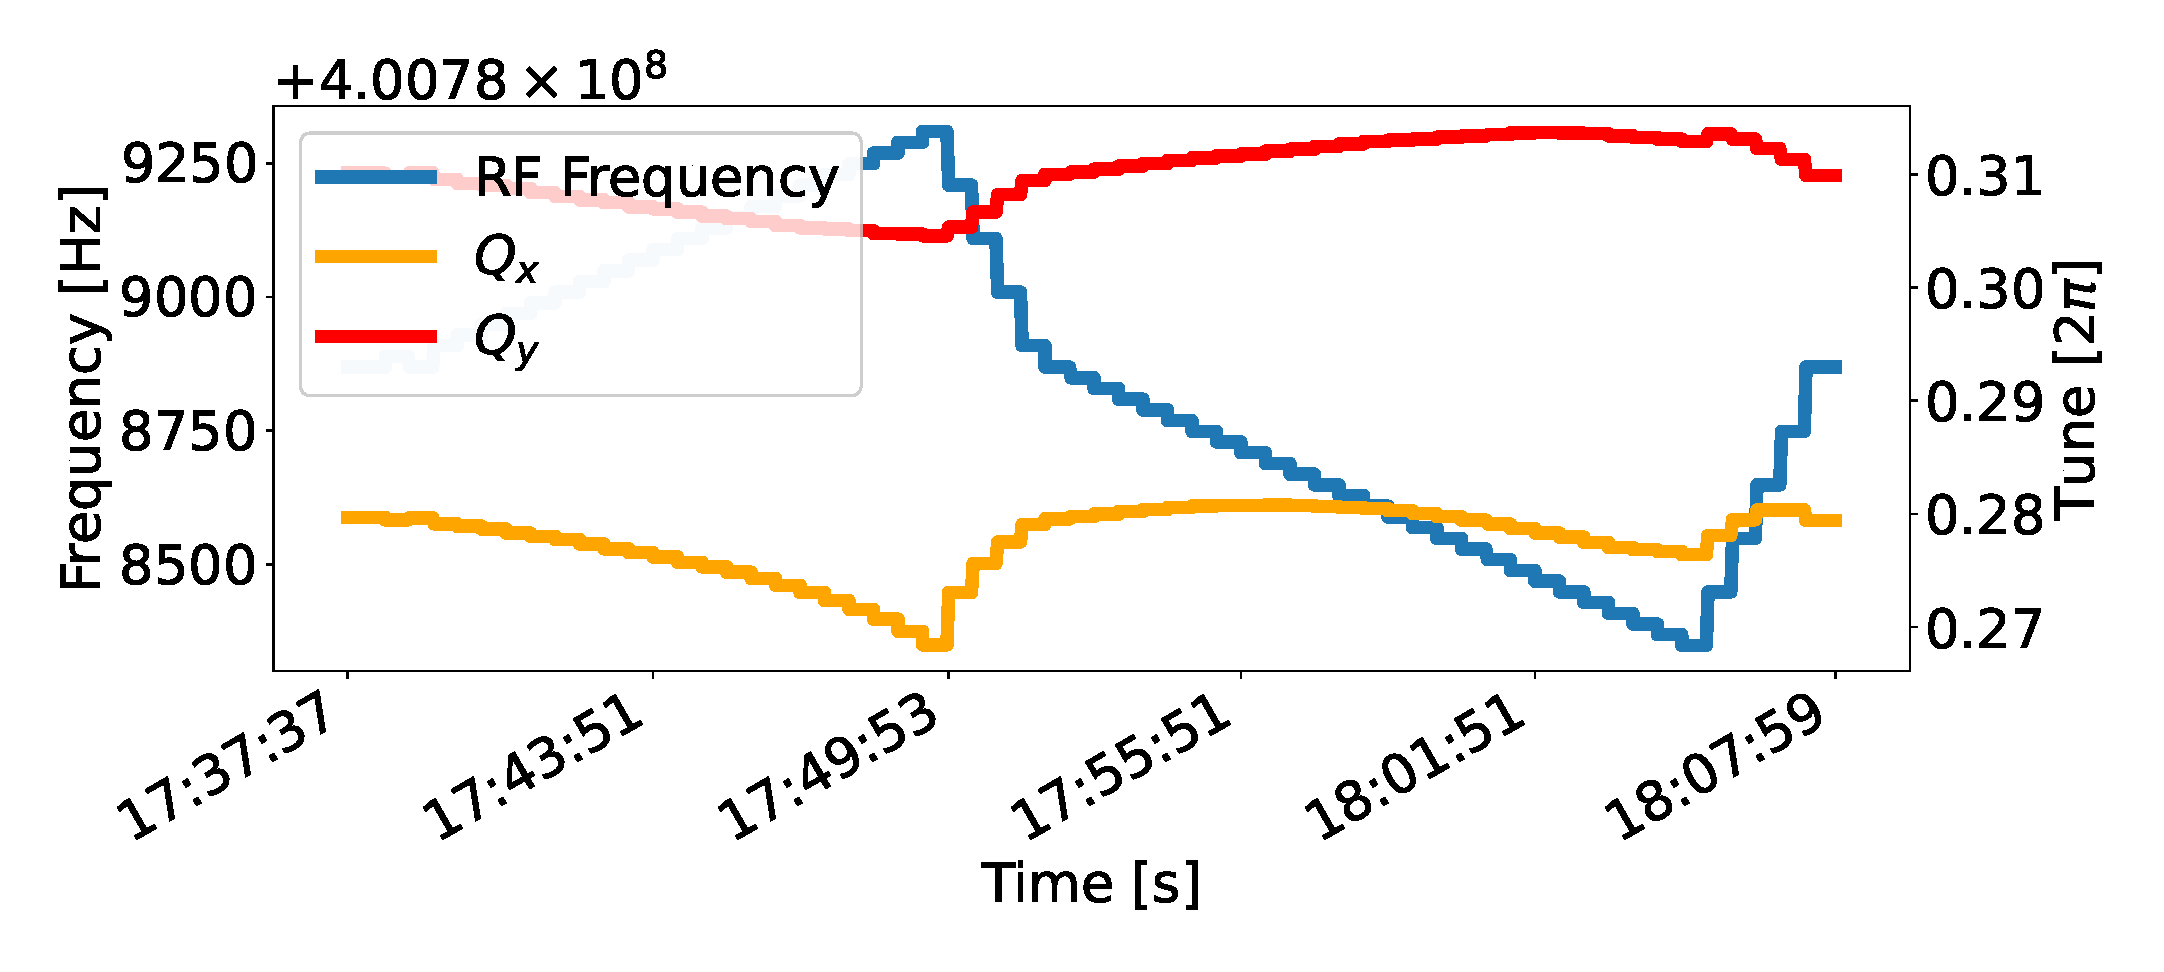
\includegraphics[width=1\textwidth]{images/rf_scan.pdf}
    \caption{Observation of the tune dependence on momentum offset, created by a shift of RF frequency}
    \label{fig:measurements:rf_scan}
\end{figure}




% --- Analysis and Fit ---
\subsubsection{Analysis}
